
% Default to the notebook output style

    


% Inherit from the specified cell style.




    
\documentclass[11pt]{article}

    
    
    \usepackage[T1]{fontenc}
    % Nicer default font (+ math font) than Computer Modern for most use cases
    \usepackage{mathpazo}

    % Basic figure setup, for now with no caption control since it's done
    % automatically by Pandoc (which extracts ![](path) syntax from Markdown).
    \usepackage{graphicx}
    % We will generate all images so they have a width \maxwidth. This means
    % that they will get their normal width if they fit onto the page, but
    % are scaled down if they would overflow the margins.
    \makeatletter
    \def\maxwidth{\ifdim\Gin@nat@width>\linewidth\linewidth
    \else\Gin@nat@width\fi}
    \makeatother
    \let\Oldincludegraphics\includegraphics
    % Set max figure width to be 80% of text width, for now hardcoded.
    \renewcommand{\includegraphics}[1]{\Oldincludegraphics[width=.8\maxwidth]{#1}}
    % Ensure that by default, figures have no caption (until we provide a
    % proper Figure object with a Caption API and a way to capture that
    % in the conversion process - todo).
    \usepackage{caption}
    \DeclareCaptionLabelFormat{nolabel}{}
    \captionsetup{labelformat=nolabel}

    \usepackage{adjustbox} % Used to constrain images to a maximum size 
    \usepackage{xcolor} % Allow colors to be defined
    \usepackage{enumerate} % Needed for markdown enumerations to work
    \usepackage{geometry} % Used to adjust the document margins
    \usepackage{amsmath} % Equations
    \usepackage{amssymb} % Equations
    \usepackage{textcomp} % defines textquotesingle
    % Hack from http://tex.stackexchange.com/a/47451/13684:
    \AtBeginDocument{%
        \def\PYZsq{\textquotesingle}% Upright quotes in Pygmentized code
    }
    \usepackage{upquote} % Upright quotes for verbatim code
    \usepackage{eurosym} % defines \euro
    \usepackage[mathletters]{ucs} % Extended unicode (utf-8) support
    \usepackage[utf8x]{inputenc} % Allow utf-8 characters in the tex document
    \usepackage{fancyvrb} % verbatim replacement that allows latex
    \usepackage{grffile} % extends the file name processing of package graphics 
                         % to support a larger range 
    % The hyperref package gives us a pdf with properly built
    % internal navigation ('pdf bookmarks' for the table of contents,
    % internal cross-reference links, web links for URLs, etc.)
    \usepackage{hyperref}
    \usepackage{longtable} % longtable support required by pandoc >1.10
    \usepackage{booktabs}  % table support for pandoc > 1.12.2
    \usepackage[inline]{enumitem} % IRkernel/repr support (it uses the enumerate* environment)
    \usepackage[normalem]{ulem} % ulem is needed to support strikethroughs (\sout)
                                % normalem makes italics be italics, not underlines
    

    
    
    % Colors for the hyperref package
    \definecolor{urlcolor}{rgb}{0,.145,.698}
    \definecolor{linkcolor}{rgb}{.71,0.21,0.01}
    \definecolor{citecolor}{rgb}{.12,.54,.11}

    % ANSI colors
    \definecolor{ansi-black}{HTML}{3E424D}
    \definecolor{ansi-black-intense}{HTML}{282C36}
    \definecolor{ansi-red}{HTML}{E75C58}
    \definecolor{ansi-red-intense}{HTML}{B22B31}
    \definecolor{ansi-green}{HTML}{00A250}
    \definecolor{ansi-green-intense}{HTML}{007427}
    \definecolor{ansi-yellow}{HTML}{DDB62B}
    \definecolor{ansi-yellow-intense}{HTML}{B27D12}
    \definecolor{ansi-blue}{HTML}{208FFB}
    \definecolor{ansi-blue-intense}{HTML}{0065CA}
    \definecolor{ansi-magenta}{HTML}{D160C4}
    \definecolor{ansi-magenta-intense}{HTML}{A03196}
    \definecolor{ansi-cyan}{HTML}{60C6C8}
    \definecolor{ansi-cyan-intense}{HTML}{258F8F}
    \definecolor{ansi-white}{HTML}{C5C1B4}
    \definecolor{ansi-white-intense}{HTML}{A1A6B2}

    % commands and environments needed by pandoc snippets
    % extracted from the output of `pandoc -s`
    \providecommand{\tightlist}{%
      \setlength{\itemsep}{0pt}\setlength{\parskip}{0pt}}
    \DefineVerbatimEnvironment{Highlighting}{Verbatim}{commandchars=\\\{\}}
    % Add ',fontsize=\small' for more characters per line
    \newenvironment{Shaded}{}{}
    \newcommand{\KeywordTok}[1]{\textcolor[rgb]{0.00,0.44,0.13}{\textbf{{#1}}}}
    \newcommand{\DataTypeTok}[1]{\textcolor[rgb]{0.56,0.13,0.00}{{#1}}}
    \newcommand{\DecValTok}[1]{\textcolor[rgb]{0.25,0.63,0.44}{{#1}}}
    \newcommand{\BaseNTok}[1]{\textcolor[rgb]{0.25,0.63,0.44}{{#1}}}
    \newcommand{\FloatTok}[1]{\textcolor[rgb]{0.25,0.63,0.44}{{#1}}}
    \newcommand{\CharTok}[1]{\textcolor[rgb]{0.25,0.44,0.63}{{#1}}}
    \newcommand{\StringTok}[1]{\textcolor[rgb]{0.25,0.44,0.63}{{#1}}}
    \newcommand{\CommentTok}[1]{\textcolor[rgb]{0.38,0.63,0.69}{\textit{{#1}}}}
    \newcommand{\OtherTok}[1]{\textcolor[rgb]{0.00,0.44,0.13}{{#1}}}
    \newcommand{\AlertTok}[1]{\textcolor[rgb]{1.00,0.00,0.00}{\textbf{{#1}}}}
    \newcommand{\FunctionTok}[1]{\textcolor[rgb]{0.02,0.16,0.49}{{#1}}}
    \newcommand{\RegionMarkerTok}[1]{{#1}}
    \newcommand{\ErrorTok}[1]{\textcolor[rgb]{1.00,0.00,0.00}{\textbf{{#1}}}}
    \newcommand{\NormalTok}[1]{{#1}}
    
    % Additional commands for more recent versions of Pandoc
    \newcommand{\ConstantTok}[1]{\textcolor[rgb]{0.53,0.00,0.00}{{#1}}}
    \newcommand{\SpecialCharTok}[1]{\textcolor[rgb]{0.25,0.44,0.63}{{#1}}}
    \newcommand{\VerbatimStringTok}[1]{\textcolor[rgb]{0.25,0.44,0.63}{{#1}}}
    \newcommand{\SpecialStringTok}[1]{\textcolor[rgb]{0.73,0.40,0.53}{{#1}}}
    \newcommand{\ImportTok}[1]{{#1}}
    \newcommand{\DocumentationTok}[1]{\textcolor[rgb]{0.73,0.13,0.13}{\textit{{#1}}}}
    \newcommand{\AnnotationTok}[1]{\textcolor[rgb]{0.38,0.63,0.69}{\textbf{\textit{{#1}}}}}
    \newcommand{\CommentVarTok}[1]{\textcolor[rgb]{0.38,0.63,0.69}{\textbf{\textit{{#1}}}}}
    \newcommand{\VariableTok}[1]{\textcolor[rgb]{0.10,0.09,0.49}{{#1}}}
    \newcommand{\ControlFlowTok}[1]{\textcolor[rgb]{0.00,0.44,0.13}{\textbf{{#1}}}}
    \newcommand{\OperatorTok}[1]{\textcolor[rgb]{0.40,0.40,0.40}{{#1}}}
    \newcommand{\BuiltInTok}[1]{{#1}}
    \newcommand{\ExtensionTok}[1]{{#1}}
    \newcommand{\PreprocessorTok}[1]{\textcolor[rgb]{0.74,0.48,0.00}{{#1}}}
    \newcommand{\AttributeTok}[1]{\textcolor[rgb]{0.49,0.56,0.16}{{#1}}}
    \newcommand{\InformationTok}[1]{\textcolor[rgb]{0.38,0.63,0.69}{\textbf{\textit{{#1}}}}}
    \newcommand{\WarningTok}[1]{\textcolor[rgb]{0.38,0.63,0.69}{\textbf{\textit{{#1}}}}}
    
    
    % Define a nice break command that doesn't care if a line doesn't already
    % exist.
    \def\br{\hspace*{\fill} \\* }
    % Math Jax compatability definitions
    \def\gt{>}
    \def\lt{<}
    % Document parameters
    \title{HW\_2-4-7\_Network-Modeling}
    
    
    

    % Pygments definitions
    
\makeatletter
\def\PY@reset{\let\PY@it=\relax \let\PY@bf=\relax%
    \let\PY@ul=\relax \let\PY@tc=\relax%
    \let\PY@bc=\relax \let\PY@ff=\relax}
\def\PY@tok#1{\csname PY@tok@#1\endcsname}
\def\PY@toks#1+{\ifx\relax#1\empty\else%
    \PY@tok{#1}\expandafter\PY@toks\fi}
\def\PY@do#1{\PY@bc{\PY@tc{\PY@ul{%
    \PY@it{\PY@bf{\PY@ff{#1}}}}}}}
\def\PY#1#2{\PY@reset\PY@toks#1+\relax+\PY@do{#2}}

\expandafter\def\csname PY@tok@w\endcsname{\def\PY@tc##1{\textcolor[rgb]{0.73,0.73,0.73}{##1}}}
\expandafter\def\csname PY@tok@c\endcsname{\let\PY@it=\textit\def\PY@tc##1{\textcolor[rgb]{0.25,0.50,0.50}{##1}}}
\expandafter\def\csname PY@tok@cp\endcsname{\def\PY@tc##1{\textcolor[rgb]{0.74,0.48,0.00}{##1}}}
\expandafter\def\csname PY@tok@k\endcsname{\let\PY@bf=\textbf\def\PY@tc##1{\textcolor[rgb]{0.00,0.50,0.00}{##1}}}
\expandafter\def\csname PY@tok@kp\endcsname{\def\PY@tc##1{\textcolor[rgb]{0.00,0.50,0.00}{##1}}}
\expandafter\def\csname PY@tok@kt\endcsname{\def\PY@tc##1{\textcolor[rgb]{0.69,0.00,0.25}{##1}}}
\expandafter\def\csname PY@tok@o\endcsname{\def\PY@tc##1{\textcolor[rgb]{0.40,0.40,0.40}{##1}}}
\expandafter\def\csname PY@tok@ow\endcsname{\let\PY@bf=\textbf\def\PY@tc##1{\textcolor[rgb]{0.67,0.13,1.00}{##1}}}
\expandafter\def\csname PY@tok@nb\endcsname{\def\PY@tc##1{\textcolor[rgb]{0.00,0.50,0.00}{##1}}}
\expandafter\def\csname PY@tok@nf\endcsname{\def\PY@tc##1{\textcolor[rgb]{0.00,0.00,1.00}{##1}}}
\expandafter\def\csname PY@tok@nc\endcsname{\let\PY@bf=\textbf\def\PY@tc##1{\textcolor[rgb]{0.00,0.00,1.00}{##1}}}
\expandafter\def\csname PY@tok@nn\endcsname{\let\PY@bf=\textbf\def\PY@tc##1{\textcolor[rgb]{0.00,0.00,1.00}{##1}}}
\expandafter\def\csname PY@tok@ne\endcsname{\let\PY@bf=\textbf\def\PY@tc##1{\textcolor[rgb]{0.82,0.25,0.23}{##1}}}
\expandafter\def\csname PY@tok@nv\endcsname{\def\PY@tc##1{\textcolor[rgb]{0.10,0.09,0.49}{##1}}}
\expandafter\def\csname PY@tok@no\endcsname{\def\PY@tc##1{\textcolor[rgb]{0.53,0.00,0.00}{##1}}}
\expandafter\def\csname PY@tok@nl\endcsname{\def\PY@tc##1{\textcolor[rgb]{0.63,0.63,0.00}{##1}}}
\expandafter\def\csname PY@tok@ni\endcsname{\let\PY@bf=\textbf\def\PY@tc##1{\textcolor[rgb]{0.60,0.60,0.60}{##1}}}
\expandafter\def\csname PY@tok@na\endcsname{\def\PY@tc##1{\textcolor[rgb]{0.49,0.56,0.16}{##1}}}
\expandafter\def\csname PY@tok@nt\endcsname{\let\PY@bf=\textbf\def\PY@tc##1{\textcolor[rgb]{0.00,0.50,0.00}{##1}}}
\expandafter\def\csname PY@tok@nd\endcsname{\def\PY@tc##1{\textcolor[rgb]{0.67,0.13,1.00}{##1}}}
\expandafter\def\csname PY@tok@s\endcsname{\def\PY@tc##1{\textcolor[rgb]{0.73,0.13,0.13}{##1}}}
\expandafter\def\csname PY@tok@sd\endcsname{\let\PY@it=\textit\def\PY@tc##1{\textcolor[rgb]{0.73,0.13,0.13}{##1}}}
\expandafter\def\csname PY@tok@si\endcsname{\let\PY@bf=\textbf\def\PY@tc##1{\textcolor[rgb]{0.73,0.40,0.53}{##1}}}
\expandafter\def\csname PY@tok@se\endcsname{\let\PY@bf=\textbf\def\PY@tc##1{\textcolor[rgb]{0.73,0.40,0.13}{##1}}}
\expandafter\def\csname PY@tok@sr\endcsname{\def\PY@tc##1{\textcolor[rgb]{0.73,0.40,0.53}{##1}}}
\expandafter\def\csname PY@tok@ss\endcsname{\def\PY@tc##1{\textcolor[rgb]{0.10,0.09,0.49}{##1}}}
\expandafter\def\csname PY@tok@sx\endcsname{\def\PY@tc##1{\textcolor[rgb]{0.00,0.50,0.00}{##1}}}
\expandafter\def\csname PY@tok@m\endcsname{\def\PY@tc##1{\textcolor[rgb]{0.40,0.40,0.40}{##1}}}
\expandafter\def\csname PY@tok@gh\endcsname{\let\PY@bf=\textbf\def\PY@tc##1{\textcolor[rgb]{0.00,0.00,0.50}{##1}}}
\expandafter\def\csname PY@tok@gu\endcsname{\let\PY@bf=\textbf\def\PY@tc##1{\textcolor[rgb]{0.50,0.00,0.50}{##1}}}
\expandafter\def\csname PY@tok@gd\endcsname{\def\PY@tc##1{\textcolor[rgb]{0.63,0.00,0.00}{##1}}}
\expandafter\def\csname PY@tok@gi\endcsname{\def\PY@tc##1{\textcolor[rgb]{0.00,0.63,0.00}{##1}}}
\expandafter\def\csname PY@tok@gr\endcsname{\def\PY@tc##1{\textcolor[rgb]{1.00,0.00,0.00}{##1}}}
\expandafter\def\csname PY@tok@ge\endcsname{\let\PY@it=\textit}
\expandafter\def\csname PY@tok@gs\endcsname{\let\PY@bf=\textbf}
\expandafter\def\csname PY@tok@gp\endcsname{\let\PY@bf=\textbf\def\PY@tc##1{\textcolor[rgb]{0.00,0.00,0.50}{##1}}}
\expandafter\def\csname PY@tok@go\endcsname{\def\PY@tc##1{\textcolor[rgb]{0.53,0.53,0.53}{##1}}}
\expandafter\def\csname PY@tok@gt\endcsname{\def\PY@tc##1{\textcolor[rgb]{0.00,0.27,0.87}{##1}}}
\expandafter\def\csname PY@tok@err\endcsname{\def\PY@bc##1{\setlength{\fboxsep}{0pt}\fcolorbox[rgb]{1.00,0.00,0.00}{1,1,1}{\strut ##1}}}
\expandafter\def\csname PY@tok@kc\endcsname{\let\PY@bf=\textbf\def\PY@tc##1{\textcolor[rgb]{0.00,0.50,0.00}{##1}}}
\expandafter\def\csname PY@tok@kd\endcsname{\let\PY@bf=\textbf\def\PY@tc##1{\textcolor[rgb]{0.00,0.50,0.00}{##1}}}
\expandafter\def\csname PY@tok@kn\endcsname{\let\PY@bf=\textbf\def\PY@tc##1{\textcolor[rgb]{0.00,0.50,0.00}{##1}}}
\expandafter\def\csname PY@tok@kr\endcsname{\let\PY@bf=\textbf\def\PY@tc##1{\textcolor[rgb]{0.00,0.50,0.00}{##1}}}
\expandafter\def\csname PY@tok@bp\endcsname{\def\PY@tc##1{\textcolor[rgb]{0.00,0.50,0.00}{##1}}}
\expandafter\def\csname PY@tok@fm\endcsname{\def\PY@tc##1{\textcolor[rgb]{0.00,0.00,1.00}{##1}}}
\expandafter\def\csname PY@tok@vc\endcsname{\def\PY@tc##1{\textcolor[rgb]{0.10,0.09,0.49}{##1}}}
\expandafter\def\csname PY@tok@vg\endcsname{\def\PY@tc##1{\textcolor[rgb]{0.10,0.09,0.49}{##1}}}
\expandafter\def\csname PY@tok@vi\endcsname{\def\PY@tc##1{\textcolor[rgb]{0.10,0.09,0.49}{##1}}}
\expandafter\def\csname PY@tok@vm\endcsname{\def\PY@tc##1{\textcolor[rgb]{0.10,0.09,0.49}{##1}}}
\expandafter\def\csname PY@tok@sa\endcsname{\def\PY@tc##1{\textcolor[rgb]{0.73,0.13,0.13}{##1}}}
\expandafter\def\csname PY@tok@sb\endcsname{\def\PY@tc##1{\textcolor[rgb]{0.73,0.13,0.13}{##1}}}
\expandafter\def\csname PY@tok@sc\endcsname{\def\PY@tc##1{\textcolor[rgb]{0.73,0.13,0.13}{##1}}}
\expandafter\def\csname PY@tok@dl\endcsname{\def\PY@tc##1{\textcolor[rgb]{0.73,0.13,0.13}{##1}}}
\expandafter\def\csname PY@tok@s2\endcsname{\def\PY@tc##1{\textcolor[rgb]{0.73,0.13,0.13}{##1}}}
\expandafter\def\csname PY@tok@sh\endcsname{\def\PY@tc##1{\textcolor[rgb]{0.73,0.13,0.13}{##1}}}
\expandafter\def\csname PY@tok@s1\endcsname{\def\PY@tc##1{\textcolor[rgb]{0.73,0.13,0.13}{##1}}}
\expandafter\def\csname PY@tok@mb\endcsname{\def\PY@tc##1{\textcolor[rgb]{0.40,0.40,0.40}{##1}}}
\expandafter\def\csname PY@tok@mf\endcsname{\def\PY@tc##1{\textcolor[rgb]{0.40,0.40,0.40}{##1}}}
\expandafter\def\csname PY@tok@mh\endcsname{\def\PY@tc##1{\textcolor[rgb]{0.40,0.40,0.40}{##1}}}
\expandafter\def\csname PY@tok@mi\endcsname{\def\PY@tc##1{\textcolor[rgb]{0.40,0.40,0.40}{##1}}}
\expandafter\def\csname PY@tok@il\endcsname{\def\PY@tc##1{\textcolor[rgb]{0.40,0.40,0.40}{##1}}}
\expandafter\def\csname PY@tok@mo\endcsname{\def\PY@tc##1{\textcolor[rgb]{0.40,0.40,0.40}{##1}}}
\expandafter\def\csname PY@tok@ch\endcsname{\let\PY@it=\textit\def\PY@tc##1{\textcolor[rgb]{0.25,0.50,0.50}{##1}}}
\expandafter\def\csname PY@tok@cm\endcsname{\let\PY@it=\textit\def\PY@tc##1{\textcolor[rgb]{0.25,0.50,0.50}{##1}}}
\expandafter\def\csname PY@tok@cpf\endcsname{\let\PY@it=\textit\def\PY@tc##1{\textcolor[rgb]{0.25,0.50,0.50}{##1}}}
\expandafter\def\csname PY@tok@c1\endcsname{\let\PY@it=\textit\def\PY@tc##1{\textcolor[rgb]{0.25,0.50,0.50}{##1}}}
\expandafter\def\csname PY@tok@cs\endcsname{\let\PY@it=\textit\def\PY@tc##1{\textcolor[rgb]{0.25,0.50,0.50}{##1}}}

\def\PYZbs{\char`\\}
\def\PYZus{\char`\_}
\def\PYZob{\char`\{}
\def\PYZcb{\char`\}}
\def\PYZca{\char`\^}
\def\PYZam{\char`\&}
\def\PYZlt{\char`\<}
\def\PYZgt{\char`\>}
\def\PYZsh{\char`\#}
\def\PYZpc{\char`\%}
\def\PYZdl{\char`\$}
\def\PYZhy{\char`\-}
\def\PYZsq{\char`\'}
\def\PYZdq{\char`\"}
\def\PYZti{\char`\~}
% for compatibility with earlier versions
\def\PYZat{@}
\def\PYZlb{[}
\def\PYZrb{]}
\makeatother


    % Exact colors from NB
    \definecolor{incolor}{rgb}{0.0, 0.0, 0.5}
    \definecolor{outcolor}{rgb}{0.545, 0.0, 0.0}



    
    % Prevent overflowing lines due to hard-to-break entities
    \sloppy 
    % Setup hyperref package
    \hypersetup{
      breaklinks=true,  % so long urls are correctly broken across lines
      colorlinks=true,
      urlcolor=urlcolor,
      linkcolor=linkcolor,
      citecolor=citecolor,
      }
    % Slightly bigger margins than the latex defaults
    
    \geometry{verbose,tmargin=1in,bmargin=1in,lmargin=1in,rmargin=1in}
    
    

    \begin{document}
    
    
    \maketitle
    
    

    
    \hypertarget{bebi5009-homework-1}{%
\section{BEBI5009 Homework 1}\label{bebi5009-homework-1}}

Student: Shao-Ting Chiu

Student ID: B03901045

Source Code on Github:
https://github.com/stevengogogo/BEBI-5009-Mathematical-Biology

Reference: B. P.Ingalls, Mathematical Modelling in Systems Biology : An
Introduction, vol.~53, no. 9. 2014.

    \hypertarget{problem-1.-network-modelling}{%
\subsection{Problem 1. Network
Modelling}\label{problem-1.-network-modelling}}

    \begin{figure}
\centering
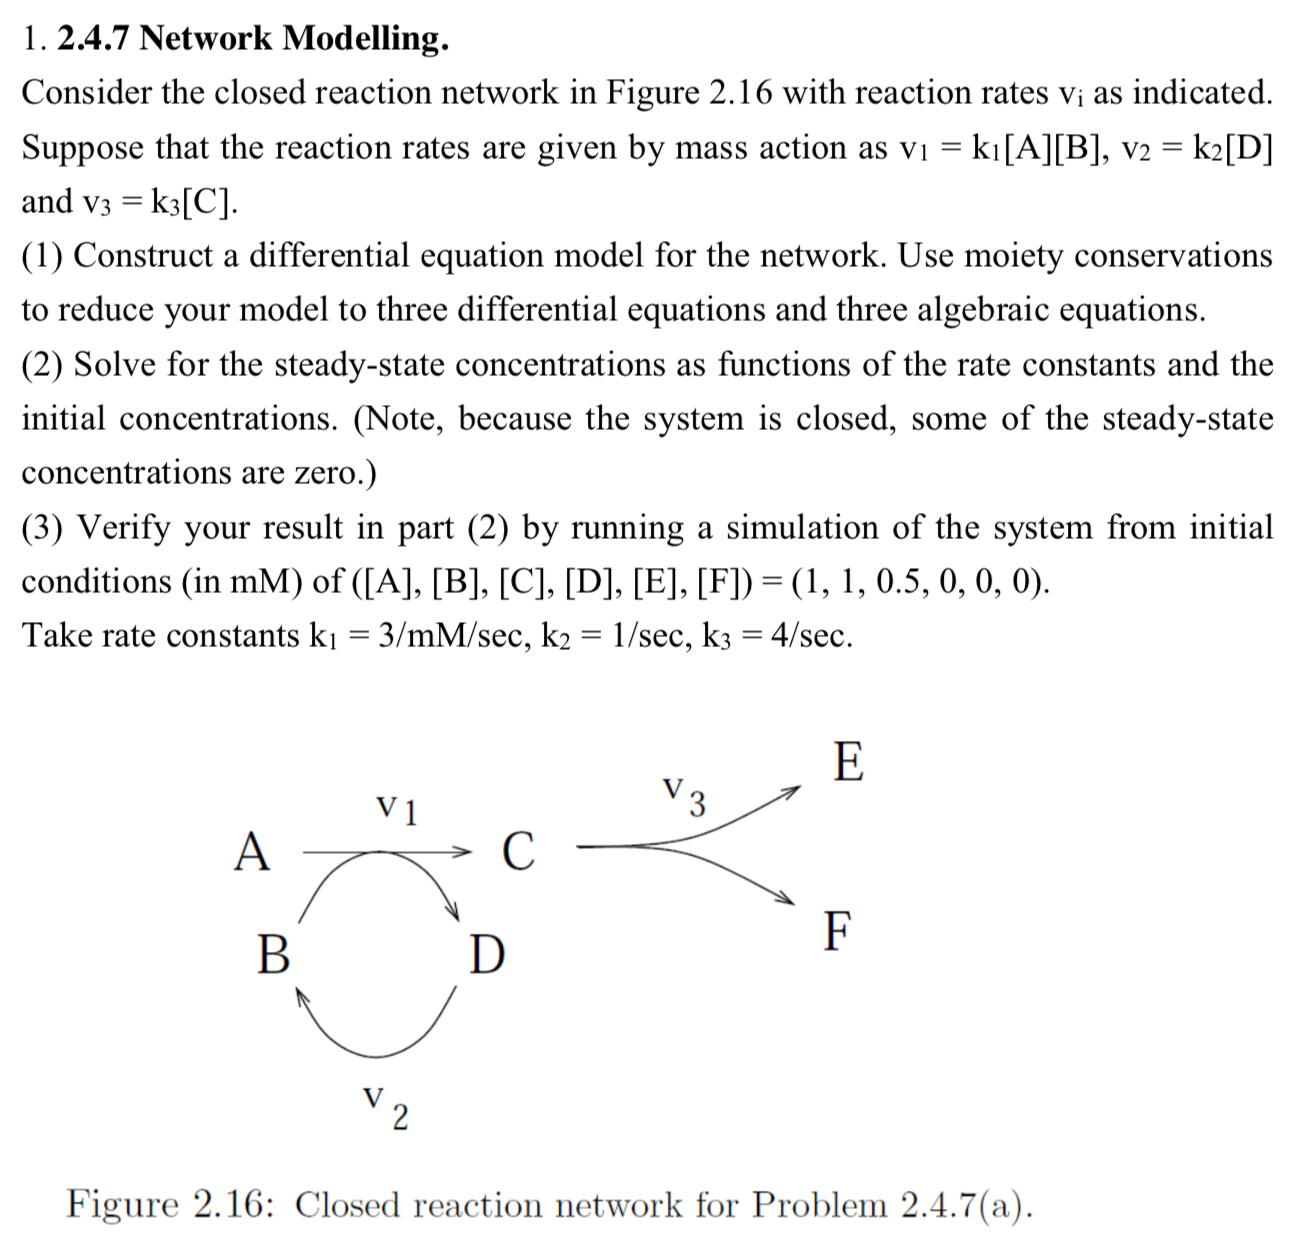
\includegraphics{img/p2-4-7.png}
\caption{Image of problem-2-4-7}
\end{figure}

    \hypertarget{a.i-construct-a-differential-equation-model-for-the-network.}{%
\subsubsection{a.i) Construct a differential equation model for the
network.}\label{a.i-construct-a-differential-equation-model-for-the-network.}}

Sol:

According the assumption in a)

\[\begin{align}
\frac{d[A]}{dt}&=-v_{1}=-k_{1}[A][B] \\
\frac{d[B]}{dt}&=-v_{1}+v_{2}=-k_{1}[A][B]+k_{2}[D] \\
\frac{d[C]}{dt}&=v_{1}-v_{3}=k_{1}[A][B]-k_{3}[C] \\
\frac{d[D]}{dt}&=v_{1}-v_{2}=k_{1}[A][B]-k_{2}[D] \\
\frac{d[E]}{dt}&=\frac{d[F]}{dt}=v_{3}=k_{3}[C] 
\end{align}\]

    Therefore, \(-\frac{d[B]}{dt}=\frac{d[D]}{dt}\);
\(-\frac{d[C]}{dt}-\frac{d[A]}{dt}=\frac{d[E]}{dt}=\frac{d[F]}{dt}\)

    We can observe that \(\frac{d[D]}{dt}\), \(\frac{d[E]}{dt}\),
\(\frac{d[F]}{dt}\) are the linear combination of set:
{[}\(\frac{d[A]}{dt},\frac{d[B]}{dt}, \frac{d[C]}{dt}\){]}. Because
\(-\frac{d[B]}{dt}=\frac{d[D]}{dt}\), \([D] = -[B]+c_{0}\), where
\(c_{0}\) is a constant. This network includes three equations and
algebraic equations, and they are

    \[\frac{d[A]}{dt}=-v_{1}=-k_{1}[A][B]\]

\[\frac{d[B]}{dt}=v_{1}-v_{2}=k_{1}[A][B]-k_{2}[D]=k_{1}[A][B]-k_{2}(-[B]+c_{0})\]

\[\frac{d[C]}{dt}=v_{1}-v_{3}=k_{1}[A][B]-k_{3}[C]\]

    \hypertarget{a.ii-solve-the-steady-state-concentration-by-rate-variables-and-initial-concentrations.}{%
\subsubsection{a.ii) Solve the steady state concentration by rate
variables and initial
concentrations.}\label{a.ii-solve-the-steady-state-concentration-by-rate-variables-and-initial-concentrations.}}

    Sol:

Under the steady state, all the chemicals will reach the dynamic
equibrilium. In other words, the derivative of chemicals in respect of
time is zero. Besides, I assume all the rate variables aren't equal to
zero.

\[\begin{align}
-k_{1}[A]^{ss}[B]^{ss}=0 \\
k_{1}[A]^{ss}[B]^{ss}-k_{2}(-[B]^{ss}+c_{0})=0 \\
k_{1}[A]^{ss}[B]^{ss}-k_{3}[C]^{ss}=0 \\
\end{align}\]

    According to the equations above, \[k_{1}[A]^{ss}[B]^{ss}=0\]

\[k_{3}[C]^{ss}=k_{1}[A]^{ss}[B]^{ss}=0\]

\[k_{2}[B]^{ss}-k_{2}c_{0}=0\]

    where \(c_{0}=[B]_{0}+[D]_{0}\)

    The steady state concentraions are: \[\begin{align}
[A]^{ss}&=0 \\
[B]^{ss}&=[B]_{t=0}+[D]_{t=0} \\
[C]^{ss}&=0 \\
[D]^{ss}&=\frac{k_1}{k_2}[A]^{ss}[B]^{ss}=0 \\
[E]^{ss}&=\int_{0}^{\infty}[C]_{t}dt+[E]_{t=0} \\
[F]^{ss}&=\int_{0}^{\infty}[C]_{t}dt+[F]_{t=0} \\
\end{align}\]

    \hypertarget{a.iii-verify-the-result-by-simulation}{%
\subsubsection{a.iii) Verify the Result by
Simulation}\label{a.iii-verify-the-result-by-simulation}}

    Here, I used Scipy ODE solver, odeint which I learned from
\href{https://docs.scipy.org/doc/scipy/reference/generated/scipy.integrate.odeint.html}{Scipy
Documentation}, and
\href{http://scipy-cookbook.readthedocs.io/items/CoupledSpringMassSystem.html}{Scipy
Cookbook}

    The following code defines the system of equations (also known as vector
field). Note that the time t must be the second argument of the
function.

    \begin{Verbatim}[commandchars=\\\{\}]
{\color{incolor}In [{\color{incolor}63}]:} \PY{k}{def} \PY{n+nf}{reaction}\PY{p}{(}\PY{n}{agent}\PY{p}{,} \PY{n}{t}\PY{p}{,} \PY{n}{k}\PY{p}{)}\PY{p}{:}
             \PY{l+s+sd}{\PYZdq{}\PYZdq{}\PYZdq{}}
         \PY{l+s+sd}{    Define the differential equations for the network system.}
         \PY{l+s+sd}{    }
         \PY{l+s+sd}{    Arguments:}
         \PY{l+s+sd}{            agent: vector of the chemical concentrations:}
         \PY{l+s+sd}{                    agent = [a,b,c,d,e,f]}
         \PY{l+s+sd}{                k: vector of rate constants:}
         \PY{l+s+sd}{                    k = [k1, k2, k3]}
         \PY{l+s+sd}{                t: time}
         \PY{l+s+sd}{    \PYZdq{}\PYZdq{}\PYZdq{}}
             \PY{n}{a}\PY{p}{,} \PY{n}{b}\PY{p}{,} \PY{n}{c}\PY{p}{,} \PY{n}{d}\PY{p}{,} \PY{n}{e}\PY{p}{,} \PY{n}{f} \PY{o}{=} \PY{n}{agent}
             \PY{n}{k1}\PY{p}{,} \PY{n}{k2}\PY{p}{,} \PY{n}{k3} \PY{o}{=} \PY{n}{k}
             
             \PY{c+c1}{\PYZsh{} Create dfdt = [a\PYZsq{}, b\PYZsq{}, c\PYZsq{}, d\PYZsq{}, e\PYZsq{}, f\PYZsq{}]:}
             \PY{n}{dfdt} \PY{o}{=} \PY{p}{[}
                     \PY{o}{\PYZhy{}}\PY{l+m+mi}{1}\PY{o}{*}\PY{n}{k1}\PY{o}{*}\PY{n}{a}\PY{o}{*}\PY{n}{b}\PY{p}{,}
                     \PY{o}{\PYZhy{}}\PY{l+m+mi}{1}\PY{o}{*}\PY{n}{k1}\PY{o}{*}\PY{n}{a}\PY{o}{*}\PY{n}{b}\PY{o}{+}\PY{n}{k2}\PY{o}{*}\PY{n}{d}\PY{p}{,}
                     \PY{n}{k1}\PY{o}{*}\PY{n}{a}\PY{o}{*}\PY{n}{b}\PY{o}{\PYZhy{}}\PY{n}{k3}\PY{o}{*}\PY{n}{c}\PY{p}{,}
                     \PY{n}{k1}\PY{o}{*}\PY{n}{a}\PY{o}{*}\PY{n}{b}\PY{o}{\PYZhy{}}\PY{n}{k2}\PY{o}{*}\PY{n}{d}\PY{p}{,}
                     \PY{n}{k3}\PY{o}{*}\PY{n}{c}\PY{p}{,}
                     \PY{n}{k3}\PY{o}{*}\PY{n}{c}
                    \PY{p}{]}
             
             \PY{k}{return} \PY{n}{dfdt}
\end{Verbatim}


    Next, here is a script that uses odeint to solve the equations for a
given set of parameter values, initial conditions, and time interval.

    \begin{Verbatim}[commandchars=\\\{\}]
{\color{incolor}In [{\color{incolor}92}]:} \PY{c+c1}{\PYZsh{} Use ODEINT to solve the differential equations defines by the vector field}
         \PY{k+kn}{import} \PY{n+nn}{numpy} \PY{k}{as} \PY{n+nn}{np}
         \PY{k+kn}{from} \PY{n+nn}{scipy}\PY{n+nn}{.}\PY{n+nn}{integrate} \PY{k}{import} \PY{n}{odeint}
         
         \PY{c+c1}{\PYZsh{} Initial condition and rate constants}
         \PY{n}{a0}\PY{p}{,} \PY{n}{b0}\PY{p}{,} \PY{n}{c0}\PY{p}{,} \PY{n}{d0}\PY{p}{,} \PY{n}{e0}\PY{p}{,} \PY{n}{f0} \PY{o}{=} \PY{l+m+mf}{1.0}\PY{p}{,} \PY{l+m+mf}{1.0}\PY{p}{,} \PY{l+m+mf}{0.5}\PY{p}{,} \PY{l+m+mf}{0.0}\PY{p}{,} \PY{l+m+mf}{0.0}\PY{p}{,} \PY{l+m+mf}{0.0} \PY{c+c1}{\PYZsh{} Initial condition}
         \PY{n}{k1}\PY{p}{,} \PY{n}{k2}\PY{p}{,} \PY{n}{k3} \PY{o}{=} \PY{l+m+mf}{3.0}\PY{p}{,} \PY{l+m+mf}{1.0}\PY{p}{,} \PY{l+m+mf}{4.0} \PY{c+c1}{\PYZsh{} Rate constants}
         
         \PY{c+c1}{\PYZsh{} Pack up the parameters and initial conditions:}
         \PY{n}{agent0} \PY{o}{=} \PY{p}{[}\PY{n}{a0}\PY{p}{,} \PY{n}{b0}\PY{p}{,} \PY{n}{c0}\PY{p}{,} \PY{n}{d0}\PY{p}{,} \PY{n}{e0}\PY{p}{,} \PY{n}{f0}\PY{p}{]}
         \PY{n}{k} \PY{o}{=} \PY{p}{[}\PY{n}{k1}\PY{p}{,} \PY{n}{k2}\PY{p}{,} \PY{n}{k3}\PY{p}{]}
         
         \PY{c+c1}{\PYZsh{} ODE solver parameters}
         \PY{n}{abserr} \PY{o}{=} \PY{l+m+mf}{1.0e\PYZhy{}8}
         \PY{n}{relerr} \PY{o}{=} \PY{l+m+mf}{1.0e\PYZhy{}6}
         \PY{n}{stoptime} \PY{o}{=} \PY{l+m+mf}{10.0}
         \PY{n}{numpoints} \PY{o}{=} \PY{l+m+mi}{500}
         
         \PY{c+c1}{\PYZsh{} Create the time samples for the output of the ODE solver.}
         \PY{n}{t} \PY{o}{=} \PY{n}{np}\PY{o}{.}\PY{n}{linspace}\PY{p}{(}\PY{l+m+mi}{0}\PY{p}{,} \PY{n}{stoptime}\PY{p}{,} \PY{n}{numpoints}\PY{p}{)}
         
         \PY{c+c1}{\PYZsh{} Call the ODE solver }
         \PY{n}{wsol} \PY{o}{=} \PY{n}{odeint}\PY{p}{(}\PY{n}{reaction}\PY{p}{,} \PY{n}{agent0}\PY{p}{,} \PY{n}{t}\PY{p}{,} \PY{n}{args}\PY{o}{=}\PY{p}{(}\PY{n}{k}\PY{p}{,}\PY{p}{)}\PY{p}{,} \PY{n}{atol}\PY{o}{=}\PY{n}{abserr}\PY{p}{,} \PY{n}{rtol}\PY{o}{=}\PY{n}{relerr}\PY{p}{)}
\end{Verbatim}


    \begin{Verbatim}[commandchars=\\\{\}]
{\color{incolor}In [{\color{incolor}96}]:} \PY{c+c1}{\PYZsh{} Check the shape of wsol (numpoints, chemicals)}
         \PY{n}{wsol}\PY{o}{.}\PY{n}{shape}
\end{Verbatim}


\begin{Verbatim}[commandchars=\\\{\}]
{\color{outcolor}Out[{\color{outcolor}96}]:} (500, 6)
\end{Verbatim}
            
    Print out the steady-state concentrations of network systmem

    \begin{Verbatim}[commandchars=\\\{\}]
{\color{incolor}In [{\color{incolor}94}]:} \PY{n}{label} \PY{o}{=} \PY{p}{[}\PY{l+s+sa}{r}\PY{l+s+s1}{\PYZsq{}}\PY{l+s+s1}{[A]}\PY{l+s+s1}{\PYZsq{}}\PY{p}{,}\PY{l+s+sa}{r}\PY{l+s+s1}{\PYZsq{}}\PY{l+s+s1}{[B]}\PY{l+s+s1}{\PYZsq{}}\PY{p}{,}\PY{l+s+sa}{r}\PY{l+s+s1}{\PYZsq{}}\PY{l+s+s1}{[C]}\PY{l+s+s1}{\PYZsq{}}\PY{p}{,}\PY{l+s+sa}{r}\PY{l+s+s1}{\PYZsq{}}\PY{l+s+s1}{[D]}\PY{l+s+s1}{\PYZsq{}}\PY{p}{,}\PY{l+s+sa}{r}\PY{l+s+s1}{\PYZsq{}}\PY{l+s+s1}{[E]}\PY{l+s+s1}{\PYZsq{}}\PY{p}{,}\PY{l+s+sa}{r}\PY{l+s+s1}{\PYZsq{}}\PY{l+s+s1}{[F]}\PY{l+s+s1}{\PYZsq{}}\PY{p}{]}
         
         \PY{c+c1}{\PYZsh{} Print out Steady\PYZhy{}state concentrations}
         \PY{n+nb}{print}\PY{p}{(}\PY{l+s+s1}{\PYZsq{}}\PY{l+s+s1}{Steady\PYZhy{}state concentration}\PY{l+s+s1}{\PYZsq{}}\PY{p}{)}
         \PY{k}{for} \PY{n}{i} \PY{o+ow}{in} \PY{n+nb}{range}\PY{p}{(}\PY{n}{wsol}\PY{o}{.}\PY{n}{shape}\PY{p}{[}\PY{l+m+mi}{1}\PY{p}{]}\PY{p}{)}\PY{p}{:}
             \PY{n+nb}{print}\PY{p}{(}\PY{n}{label}\PY{p}{[}\PY{n}{i}\PY{p}{]}\PY{p}{,}\PY{l+s+s1}{\PYZsq{}}\PY{l+s+s1}{: }\PY{l+s+s1}{\PYZsq{}}\PY{p}{,}\PY{n+nb}{round}\PY{p}{(}\PY{n}{wsol}\PY{p}{[}\PY{o}{\PYZhy{}}\PY{l+m+mi}{1}\PY{p}{,}\PY{n}{i}\PY{p}{]}\PY{p}{,} \PY{l+m+mi}{2}\PY{p}{)}\PY{p}{,}\PY{l+s+s1}{\PYZsq{}}\PY{l+s+se}{\PYZbs{}t}\PY{l+s+s1}{mM}\PY{l+s+s1}{\PYZsq{}}\PY{p}{)}
             
\end{Verbatim}


    \begin{Verbatim}[commandchars=\\\{\}]
Steady-state concentration
[A] :  0.0 	mM
[B] :  1.0 	mM
[C] :  0.0 	mM
[D] :  0.0 	mM
[E] :  1.5 	mM
[F] :  1.5 	mM

    \end{Verbatim}

    The following script uses Matplotlib to plot the solution generated by
the above script.

    \begin{Verbatim}[commandchars=\\\{\}]
{\color{incolor}In [{\color{incolor}95}]:} \PY{k+kn}{import} \PY{n+nn}{matplotlib}\PY{n+nn}{.}\PY{n+nn}{pyplot} \PY{k}{as} \PY{n+nn}{plt}
         
         \PY{n}{fig\PYZus{}reaction} \PY{o}{=} \PY{n}{plt}\PY{o}{.}\PY{n}{figure}\PY{p}{(}\PY{p}{)}
         
         \PY{k}{for} \PY{n}{i} \PY{o+ow}{in} \PY{n+nb}{range}\PY{p}{(}\PY{n}{wsol}\PY{o}{.}\PY{n}{shape}\PY{p}{[}\PY{l+m+mi}{1}\PY{p}{]}\PY{p}{)}\PY{p}{:}
             \PY{n}{plt}\PY{o}{.}\PY{n}{plot}\PY{p}{(}\PY{n}{t}\PY{p}{,}\PY{n}{wsol}\PY{p}{[}\PY{p}{:}\PY{p}{,}\PY{n}{i}\PY{p}{]}\PY{p}{,} \PY{n}{label}\PY{o}{=}\PY{n}{label}\PY{p}{[}\PY{n}{i}\PY{p}{]}\PY{p}{)}
         
         \PY{n}{plt}\PY{o}{.}\PY{n}{legend}\PY{p}{(}\PY{p}{)}
         \PY{n}{plt}\PY{o}{.}\PY{n}{grid}\PY{p}{(}\PY{p}{)}
         \PY{n}{plt}\PY{o}{.}\PY{n}{title}\PY{p}{(}\PY{l+s+s1}{\PYZsq{}}\PY{l+s+s1}{Reaction of Network System}\PY{l+s+s1}{\PYZsq{}}\PY{p}{)}
         \PY{n}{plt}\PY{o}{.}\PY{n}{xlabel}\PY{p}{(}\PY{l+s+s1}{\PYZsq{}}\PY{l+s+s1}{time (second)}\PY{l+s+s1}{\PYZsq{}}\PY{p}{)}
         \PY{n}{plt}\PY{o}{.}\PY{n}{ylabel}\PY{p}{(}\PY{l+s+s1}{\PYZsq{}}\PY{l+s+s1}{Concentration(mM)}\PY{l+s+s1}{\PYZsq{}}\PY{p}{)}
\end{Verbatim}


\begin{Verbatim}[commandchars=\\\{\}]
{\color{outcolor}Out[{\color{outcolor}95}]:} Text(0,0.5,'Concentration(mM)')
\end{Verbatim}
            
    \begin{center}
    \adjustimage{max size={0.9\linewidth}{0.9\paperheight}}{output_22_1.png}
    \end{center}
    { \hspace*{\fill} \\}
    
    According to the results, \([A]^{ss}=[C]^{ss}=[D]^{ss}=0\),
\([B]^{ss}=[B]_0+[D]_0=1+0\), \([E]^{ss}=[F]^{ss}=1.5mM\) which mutually
support the calculation in a.ii). Besides, the solver even told us the
value of \([E]^{ss}\) and \([F]^{ss}\). In conclusion, the simulation
support the paper-and-pancil calculation of a.i), and a.ii).

    \hypertarget{problem-2.-numerical-methid-fourth-order-runge-kutta-method-rk4}{%
\subsection{Problem 2. Numerical methid: Fourth-order Runge Kutta Method
(RK4)}\label{problem-2.-numerical-methid-fourth-order-runge-kutta-method-rk4}}

SAMPLE CODE: https://github.com/SosirisTseng/BEBI-5009/tree/master/ch2

    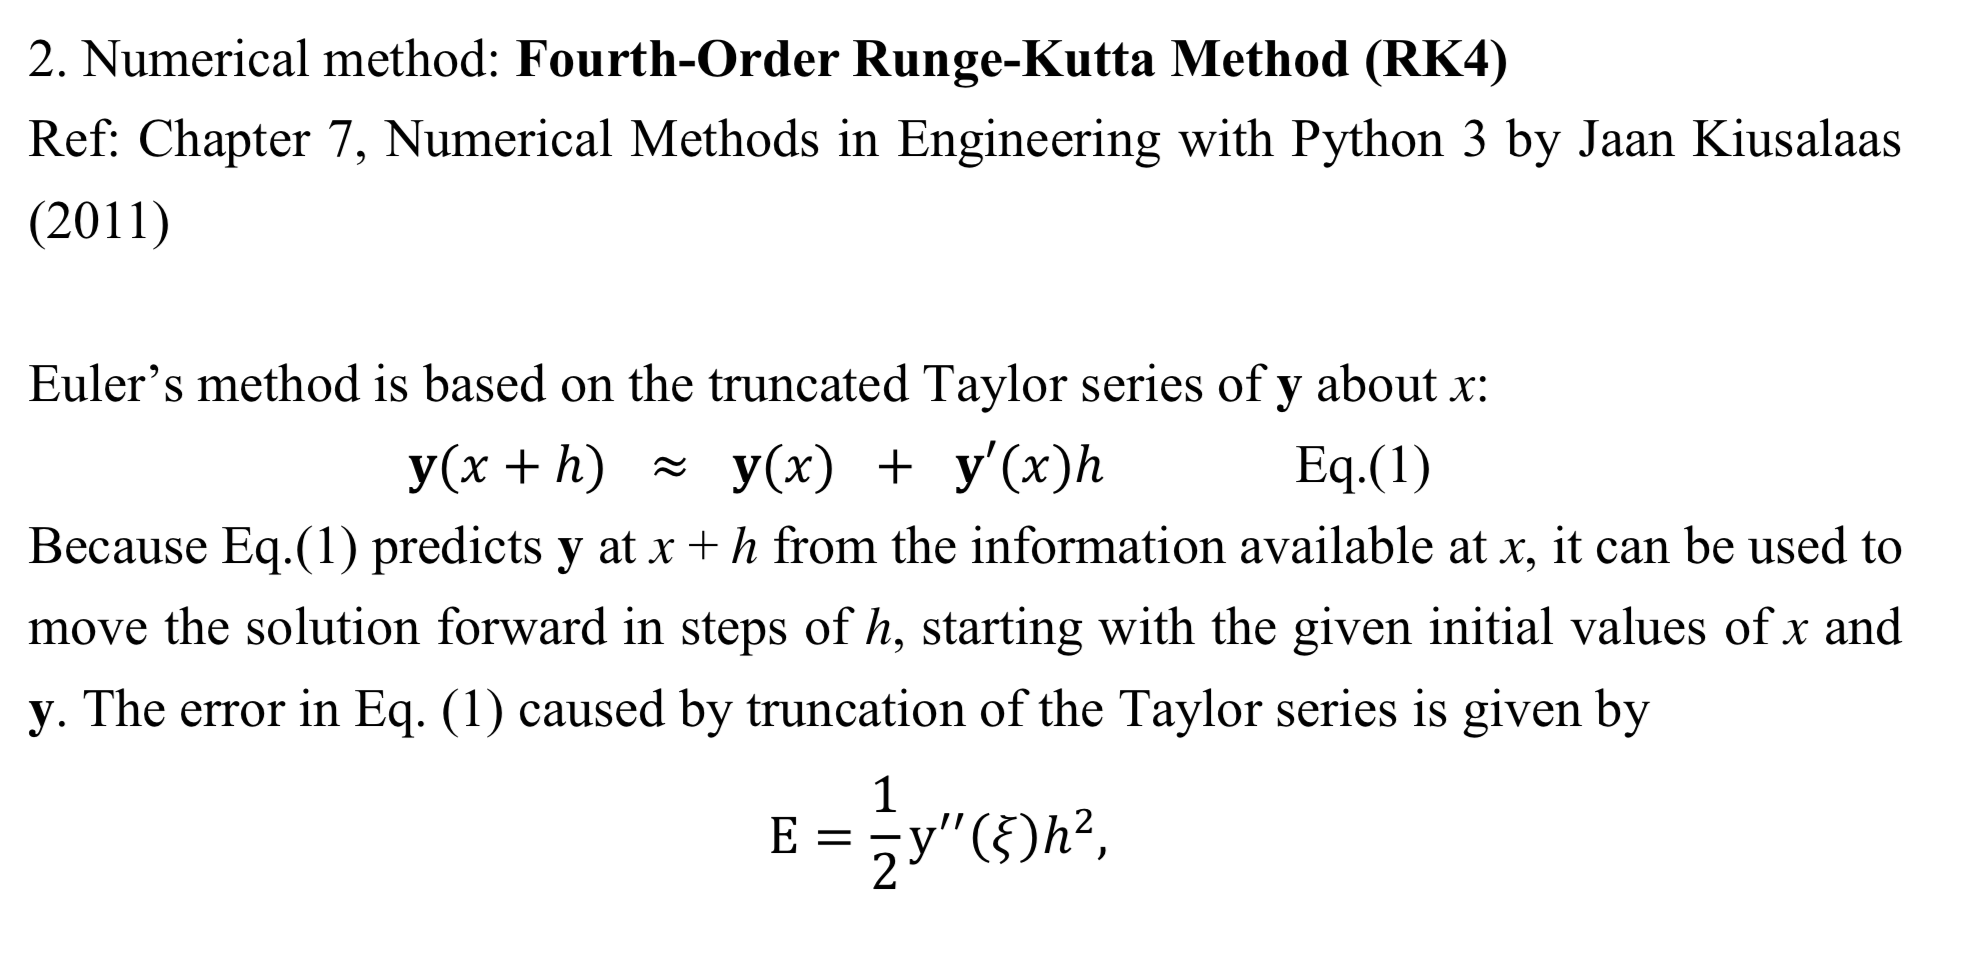
\includegraphics{img/p2-1-RK4.png} 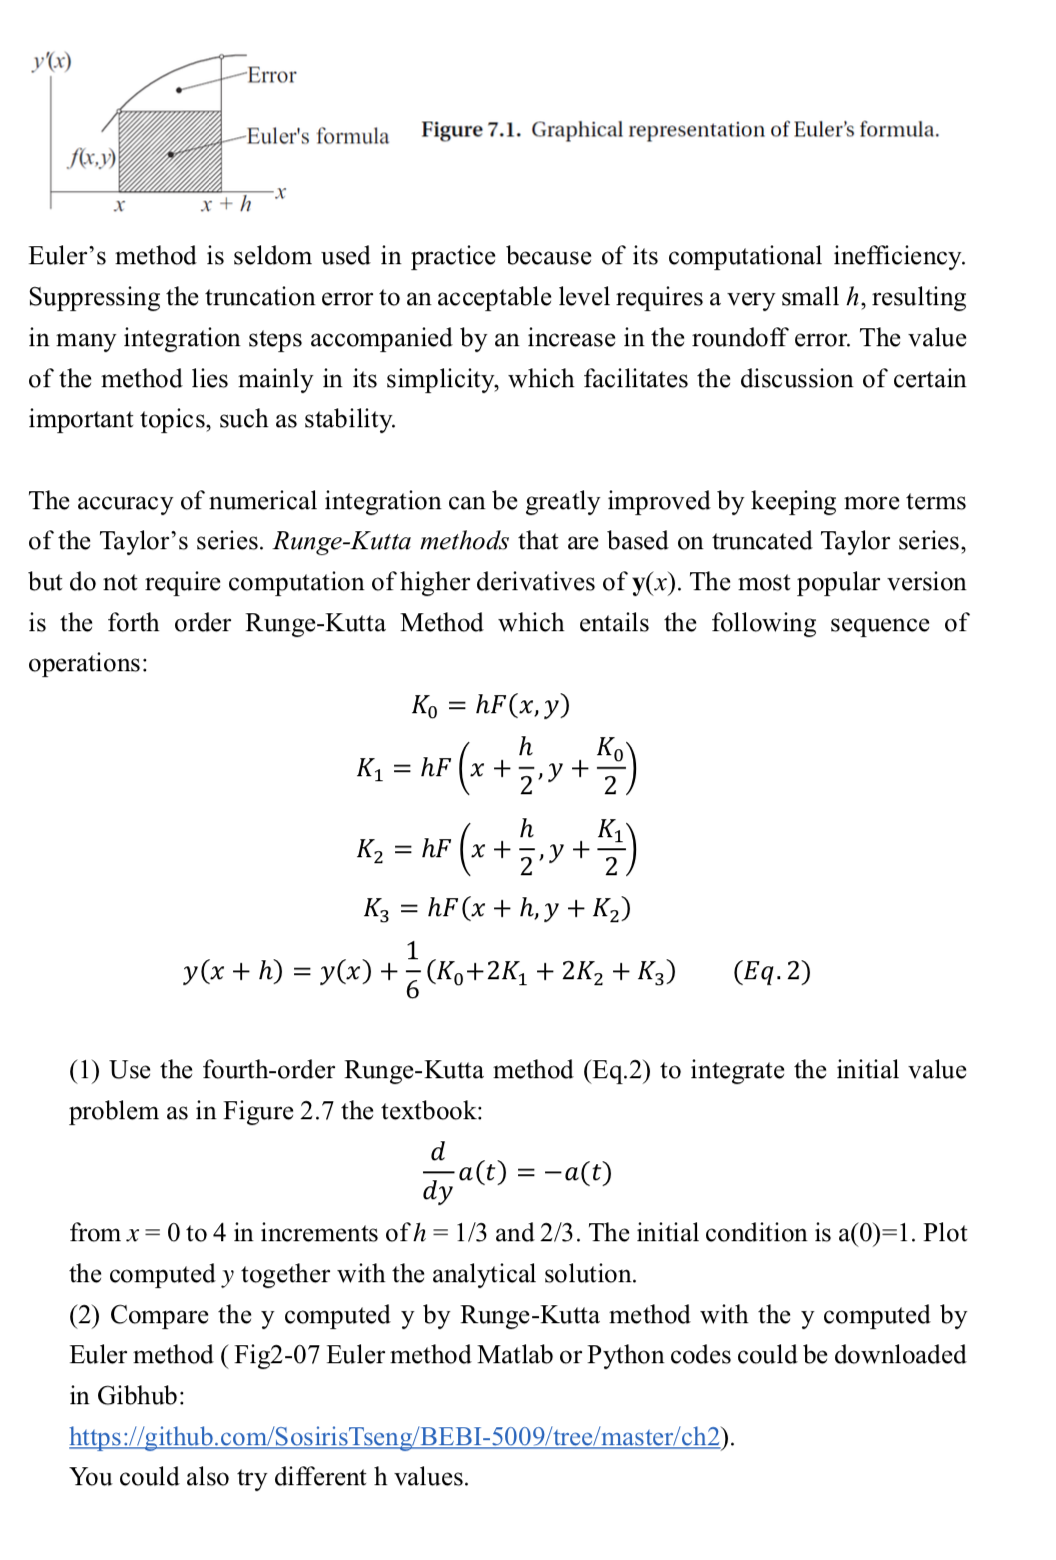
\includegraphics{img/p2-2-RK4.png}

    Sol:

    \hypertarget{analytical-solution}{%
\subsubsection{2.1 Analytical Solution}\label{analytical-solution}}

\(\frac{da(t)}{dt}=-a(t)\) is an autonomous equation. It can be solved
by ``integral-by-part'' method:

\[\begin{align}
    \frac{da(t)}{dt} &= -a(a) \\
    \frac{-1}{a(t)}da(t) &= dt \\
    \int\frac{-1}{a(t)}da(t) &= \int dt \\
    -ln(a(t)) &= t + c_{0} \\
    a(t) &= c_{1}e^{-t} \\
\end{align}\]

where \(c_{0}\) and \(c_{1}\) are constants.

With initial condition \(a(0)=1\):

\[\begin{align}
    a(t)=e^{-t}
\end{align}\]

    \hypertarget{numerical-solution}{%
\subsubsection{2.2 Numerical Solution}\label{numerical-solution}}

In the following code, both RK and Euler method are implemented and
wrapped inside an object-class. In the beginning, I define the automous
ODE in a Python function.

    \begin{Verbatim}[commandchars=\\\{\}]
{\color{incolor}In [{\color{incolor}2}]:} \PY{k}{def} \PY{n+nf}{autoODE}\PY{p}{(}\PY{n}{a}\PY{p}{,} \PY{n}{t}\PY{p}{)}\PY{p}{:}
            \PY{l+s+sd}{\PYZdq{}\PYZdq{}\PYZdq{}}
        \PY{l+s+sd}{    Define the differential equations.}
        \PY{l+s+sd}{    }
        \PY{l+s+sd}{    Arguments:}
        \PY{l+s+sd}{            a: variable}
        \PY{l+s+sd}{            t: time}
        \PY{l+s+sd}{    \PYZdq{}\PYZdq{}\PYZdq{}}
            \PY{c+c1}{\PYZsh{} Create dfdt = [a\PYZsq{}]:}
            \PY{n}{dfdt} \PY{o}{=} \PY{p}{[}
                    \PY{o}{\PYZhy{}}\PY{n}{a}
                   \PY{p}{]}
            
            \PY{k}{return} \PY{n}{dfdt}
\end{Verbatim}


    Second, I created an Python class including RK and Euler ODE solver,
which provides flexibility for future add-ons.

    \begin{Verbatim}[commandchars=\\\{\}]
{\color{incolor}In [{\color{incolor}3}]:} \PY{k}{class} \PY{n+nc}{ode\PYZus{}equation}\PY{p}{:}
            \PY{l+s+sd}{\PYZdq{}\PYZdq{}\PYZdq{}}
        \PY{l+s+sd}{    Class object provide RK estimation for ODE equation}
        \PY{l+s+sd}{    }
        \PY{l+s+sd}{    Functions:}
        \PY{l+s+sd}{        \PYZus{}\PYZus{}init\PYZus{}\PYZus{}}
        \PY{l+s+sd}{        iteration}
        \PY{l+s+sd}{        rk\PYZus{}step}
        \PY{l+s+sd}{        k}
        \PY{l+s+sd}{        euler\PYZus{}step}
        \PY{l+s+sd}{    \PYZdq{}\PYZdq{}\PYZdq{}}
            \PY{k}{def} \PY{n+nf}{\PYZus{}\PYZus{}init\PYZus{}\PYZus{}}\PY{p}{(}\PY{n+nb+bp}{self}\PY{p}{,} \PY{n}{equation}\PY{p}{)}\PY{p}{:}
                \PY{l+s+sd}{\PYZdq{}\PYZdq{}\PYZdq{}}
        \PY{l+s+sd}{        f(a) = da/dt}
        \PY{l+s+sd}{        \PYZdq{}\PYZdq{}\PYZdq{}}
                \PY{n+nb+bp}{self}\PY{o}{.}\PY{n}{equation} \PY{o}{=} \PY{n}{equation} \PY{c+c1}{\PYZsh{} Store the ODE function}
                
            \PY{k}{def} \PY{n+nf}{iteration}\PY{p}{(}\PY{n+nb+bp}{self}\PY{p}{,} \PY{n}{init}\PY{o}{=}\PY{l+m+mi}{1}\PY{p}{,} \PY{n}{start}\PY{o}{=}\PY{l+m+mi}{0}\PY{p}{,} \PY{n}{end}\PY{o}{=}\PY{l+m+mi}{4}\PY{p}{,} \PY{n}{h}\PY{o}{=}\PY{l+m+mi}{1}\PY{o}{/}\PY{l+m+mf}{3.0}\PY{p}{,} \PY{n}{method}\PY{o}{=}\PY{l+s+s1}{\PYZsq{}}\PY{l+s+s1}{rk}\PY{l+s+s1}{\PYZsq{}}\PY{p}{)}\PY{p}{:}
                \PY{l+s+sd}{\PYZdq{}\PYZdq{}\PYZdq{}}
        \PY{l+s+sd}{        Using iteration process to simulate the ODE equation}
        \PY{l+s+sd}{        }
        \PY{l+s+sd}{        Arguments:}
        \PY{l+s+sd}{                init: initial value, a(0)}
        \PY{l+s+sd}{                start: start time}
        \PY{l+s+sd}{                end: end time}
        \PY{l+s+sd}{                h: step size}
        \PY{l+s+sd}{        \PYZdq{}\PYZdq{}\PYZdq{}}
                
                \PY{c+c1}{\PYZsh{} Set time step and to store iteration process}
                \PY{c+c1}{\PYZsh{} h\PYZus{}r is the real step. Approximately equal to h}
                \PY{n+nb+bp}{self}\PY{o}{.}\PY{n}{t}\PY{p}{,} \PY{n}{h\PYZus{}r} \PY{o}{=} \PY{n}{np}\PY{o}{.}\PY{n}{linspace}\PY{p}{(}\PY{n}{start}\PY{p}{,} \PY{n}{end}\PY{p}{,} \PY{n+nb}{int}\PY{p}{(}\PY{p}{(}\PY{n}{end}\PY{o}{\PYZhy{}}\PY{n}{start}\PY{p}{)}\PY{o}{/}\PY{n}{h}\PY{p}{)}\PY{p}{,} \PY{n}{retstep}\PY{o}{=}\PY{k+kc}{True}\PY{p}{)}
                \PY{n+nb+bp}{self}\PY{o}{.}\PY{n}{a} \PY{o}{=} \PY{p}{[}\PY{p}{]} 
                
                \PY{c+c1}{\PYZsh{} Set initial value}
                \PY{n+nb+bp}{self}\PY{o}{.}\PY{n}{a}\PY{o}{.}\PY{n}{append}\PY{p}{(}\PY{n}{init}\PY{p}{)}
                
                \PY{c+c1}{\PYZsh{} Iteration process }
                \PY{k}{for} \PY{n}{i}\PY{p}{,} \PY{n}{time} \PY{o+ow}{in} \PY{n+nb}{enumerate}\PY{p}{(}\PY{n+nb+bp}{self}\PY{o}{.}\PY{n}{t}\PY{p}{[}\PY{l+m+mi}{1}\PY{p}{:}\PY{p}{]}\PY{p}{)}\PY{p}{:}
                    
                    \PY{k}{if} \PY{n}{method} \PY{o}{==} \PY{l+s+s1}{\PYZsq{}}\PY{l+s+s1}{rk}\PY{l+s+s1}{\PYZsq{}}\PY{p}{:}
                        \PY{n}{a\PYZus{}next} \PY{o}{=} \PY{n+nb+bp}{self}\PY{o}{.}\PY{n}{a}\PY{p}{[}\PY{n}{i}\PY{p}{]} \PY{o}{+} \PY{n+nb+bp}{self}\PY{o}{.}\PY{n}{rk\PYZus{}step}\PY{p}{(}\PY{n+nb+bp}{self}\PY{o}{.}\PY{n}{a}\PY{p}{[}\PY{n}{i}\PY{p}{]}\PY{p}{,} \PY{n}{time}\PY{p}{,} \PY{n}{h\PYZus{}r}\PY{p}{)}
                        
                    \PY{k}{elif} \PY{n}{method} \PY{o}{==} \PY{l+s+s1}{\PYZsq{}}\PY{l+s+s1}{euler}\PY{l+s+s1}{\PYZsq{}}\PY{p}{:}
                        \PY{n}{a\PYZus{}next} \PY{o}{=} \PY{n+nb+bp}{self}\PY{o}{.}\PY{n}{a}\PY{p}{[}\PY{n}{i}\PY{p}{]} \PY{o}{+} \PY{n+nb+bp}{self}\PY{o}{.}\PY{n}{euler\PYZus{}step}\PY{p}{(}\PY{n+nb+bp}{self}\PY{o}{.}\PY{n}{a}\PY{p}{[}\PY{n}{i}\PY{p}{]}\PY{p}{,} \PY{n}{time}\PY{p}{,} \PY{n}{h\PYZus{}r}\PY{p}{)}
                        
                    \PY{k}{else}\PY{p}{:}
                        \PY{k}{raise} \PY{n+ne}{ValueError}\PY{p}{(}\PY{l+s+s1}{\PYZsq{}}\PY{l+s+s1}{This class only provides rk and euler Method}\PY{l+s+s1}{\PYZsq{}}\PY{p}{)}
                        
                    \PY{n+nb+bp}{self}\PY{o}{.}\PY{n}{a}\PY{o}{.}\PY{n}{append}\PY{p}{(}\PY{n}{a\PYZus{}next}\PY{p}{)} \PY{c+c1}{\PYZsh{} Add current step}
                    
                \PY{k}{return} \PY{n+nb+bp}{self}\PY{o}{.}\PY{n}{a}\PY{p}{,} \PY{n+nb+bp}{self}\PY{o}{.}\PY{n}{t}\PY{p}{,} \PY{n}{h\PYZus{}r}
                    
                
                
            \PY{k}{def} \PY{n+nf}{rk\PYZus{}step}\PY{p}{(}\PY{n+nb+bp}{self}\PY{p}{,} \PY{n}{a}\PY{p}{,} \PY{n}{t}\PY{p}{,} \PY{n}{h}\PY{p}{)}\PY{p}{:}
                \PY{l+s+sd}{\PYZdq{}\PYZdq{}\PYZdq{}}
        \PY{l+s+sd}{        Return one step difference by Rung\PYZhy{}Kutta Method.}
        \PY{l+s+sd}{        }
        \PY{l+s+sd}{        Arguments:}
        \PY{l+s+sd}{                a: a(t) value}
        \PY{l+s+sd}{                t: current time}
        \PY{l+s+sd}{                h: step size}
        \PY{l+s+sd}{        \PYZdq{}\PYZdq{}\PYZdq{}}
                \PY{n}{k0}\PY{p}{,} \PY{n}{k1}\PY{p}{,} \PY{n}{k2}\PY{p}{,} \PY{n}{k3} \PY{o}{=} \PY{n+nb+bp}{self}\PY{o}{.}\PY{n}{k}\PY{p}{(}\PY{n}{a}\PY{p}{,} \PY{n}{t}\PY{p}{,} \PY{n}{h}\PY{p}{)}
                \PY{k}{return} \PY{p}{(}\PY{l+m+mi}{1}\PY{o}{/}\PY{l+m+mf}{6.0}\PY{p}{)}\PY{o}{*}\PY{p}{(} \PY{n}{k0} \PY{o}{+} \PY{l+m+mi}{2}\PY{o}{*}\PY{n}{k1} \PY{o}{+} \PY{l+m+mi}{2}\PY{o}{*}\PY{n}{k2} \PY{o}{+} \PY{n}{k3} \PY{p}{)}
            
            \PY{k}{def} \PY{n+nf}{k}\PY{p}{(}\PY{n+nb+bp}{self}\PY{p}{,} \PY{n}{a}\PY{p}{,} \PY{n}{t}\PY{p}{,} \PY{n}{h}\PY{p}{)}\PY{p}{:}
                \PY{l+s+sd}{\PYZdq{}\PYZdq{}\PYZdq{}}
        \PY{l+s+sd}{        Calculate k of 3 order }
        \PY{l+s+sd}{        }
        \PY{l+s+sd}{        Arguments:}
        \PY{l+s+sd}{                a: value at a(t)}
        \PY{l+s+sd}{                t: time}
        \PY{l+s+sd}{                h: step size}
        \PY{l+s+sd}{        \PYZdq{}\PYZdq{}\PYZdq{}}
                
                \PY{n}{k0} \PY{o}{=} \PY{n}{h}\PY{o}{*}\PY{n+nb+bp}{self}\PY{o}{.}\PY{n}{equation}\PY{p}{(}\PY{n}{a}\PY{p}{,} \PY{n}{t}\PY{p}{)}\PY{p}{[}\PY{l+m+mi}{0}\PY{p}{]}
                \PY{n}{k1} \PY{o}{=} \PY{n}{h}\PY{o}{*}\PY{n+nb+bp}{self}\PY{o}{.}\PY{n}{equation}\PY{p}{(}\PY{n}{a} \PY{o}{+} \PY{n}{k0}\PY{o}{/}\PY{l+m+mf}{2.0}\PY{p}{,} \PY{n}{t} \PY{o}{+} \PY{n}{h}\PY{o}{/}\PY{l+m+mf}{2.0}\PY{p}{)}\PY{p}{[}\PY{l+m+mi}{0}\PY{p}{]}
                \PY{n}{k2} \PY{o}{=} \PY{n}{h}\PY{o}{*}\PY{n+nb+bp}{self}\PY{o}{.}\PY{n}{equation}\PY{p}{(}\PY{n}{a} \PY{o}{+} \PY{n}{k1}\PY{o}{/}\PY{l+m+mf}{2.0}\PY{p}{,} \PY{n}{t} \PY{o}{+} \PY{n}{h}\PY{o}{/}\PY{l+m+mf}{2.0}\PY{p}{)}\PY{p}{[}\PY{l+m+mi}{0}\PY{p}{]}
                \PY{n}{k3} \PY{o}{=} \PY{n}{h}\PY{o}{*}\PY{n+nb+bp}{self}\PY{o}{.}\PY{n}{equation}\PY{p}{(}\PY{n}{a} \PY{o}{+} \PY{n}{k2}\PY{p}{,} \PY{n}{t} \PY{o}{+} \PY{n}{h}\PY{p}{)}\PY{p}{[}\PY{l+m+mi}{0}\PY{p}{]}
                
                \PY{k}{return} \PY{p}{[}\PY{n}{k0}\PY{p}{,} \PY{n}{k1}\PY{p}{,} \PY{n}{k2}\PY{p}{,} \PY{n}{k3}\PY{p}{]}
            
            \PY{k}{def} \PY{n+nf}{euler\PYZus{}step}\PY{p}{(}\PY{n+nb+bp}{self}\PY{p}{,} \PY{n}{a}\PY{p}{,} \PY{n}{t}\PY{p}{,} \PY{n}{h}\PY{p}{)}\PY{p}{:}
                \PY{l+s+sd}{\PYZdq{}\PYZdq{}\PYZdq{}}
        \PY{l+s+sd}{        Return one step difference by Euler Method.}
        \PY{l+s+sd}{        }
        \PY{l+s+sd}{        Arguments:}
        \PY{l+s+sd}{                a: a(t) value}
        \PY{l+s+sd}{                t: current time}
        \PY{l+s+sd}{                h: step size}
        \PY{l+s+sd}{        \PYZdq{}\PYZdq{}\PYZdq{}}
                \PY{k}{return} \PY{n}{h}\PY{o}{*}\PY{n+nb+bp}{self}\PY{o}{.}\PY{n}{equation}\PY{p}{(}\PY{n}{a}\PY{p}{,}\PY{n}{t}\PY{p}{)}\PY{p}{[}\PY{l+m+mi}{0}\PY{p}{]}
\end{Verbatim}


    Then, create a ode solver which has defined above, and input parameters
given in the question.

    \begin{Verbatim}[commandchars=\\\{\}]
{\color{incolor}In [{\color{incolor}4}]:} \PY{k+kn}{import} \PY{n+nn}{numpy} \PY{k}{as} \PY{n+nn}{np}
        
        \PY{c+c1}{\PYZsh{} Set the ODE equation}
        \PY{n}{ode} \PY{o}{=} \PY{n}{ode\PYZus{}equation}\PY{p}{(}\PY{n}{autoODE}\PY{p}{)}
        
        \PY{c+c1}{\PYZsh{} Analytical Solution}
        \PY{n}{t\PYZus{}ana} \PY{o}{=} \PY{n}{np}\PY{o}{.}\PY{n}{linspace}\PY{p}{(}\PY{l+m+mi}{0}\PY{p}{,} \PY{l+m+mi}{4}\PY{p}{,} \PY{n+nb}{int}\PY{p}{(}\PY{p}{(}\PY{l+m+mi}{4}\PY{o}{\PYZhy{}}\PY{l+m+mi}{0}\PY{p}{)}\PY{o}{/}\PY{p}{(}\PY{l+m+mi}{1}\PY{o}{/}\PY{l+m+mf}{3.0}\PY{p}{)}\PY{p}{)}\PY{p}{)}
        \PY{n}{a\PYZus{}ana} \PY{o}{=} \PY{n}{np}\PY{o}{.}\PY{n}{exp}\PY{p}{(}\PY{o}{\PYZhy{}}\PY{n}{t\PYZus{}ana}\PY{p}{)}
        
        \PY{c+c1}{\PYZsh{} Approximate by RK }
        \PY{n}{a1}\PY{p}{,} \PY{n}{t1}\PY{p}{,} \PY{n}{h1} \PY{o}{=} \PY{n}{ode}\PY{o}{.}\PY{n}{iteration}\PY{p}{(}\PY{n}{init}\PY{o}{=}\PY{l+m+mi}{1}\PY{p}{,} \PY{n}{start}\PY{o}{=}\PY{l+m+mi}{0}\PY{p}{,} \PY{n}{end}\PY{o}{=}\PY{l+m+mi}{4}\PY{p}{,} \PY{n}{h}\PY{o}{=}\PY{l+m+mi}{1}\PY{o}{/}\PY{l+m+mf}{3.0}\PY{p}{,} \PY{n}{method}\PY{o}{=}\PY{l+s+s1}{\PYZsq{}}\PY{l+s+s1}{rk}\PY{l+s+s1}{\PYZsq{}}\PY{p}{)}
        \PY{n}{a2}\PY{p}{,} \PY{n}{t2}\PY{p}{,} \PY{n}{h2} \PY{o}{=} \PY{n}{ode}\PY{o}{.}\PY{n}{iteration}\PY{p}{(}\PY{n}{init}\PY{o}{=}\PY{l+m+mi}{1}\PY{p}{,} \PY{n}{start}\PY{o}{=}\PY{l+m+mi}{0}\PY{p}{,} \PY{n}{end}\PY{o}{=}\PY{l+m+mi}{4}\PY{p}{,} \PY{n}{h}\PY{o}{=}\PY{l+m+mi}{2}\PY{o}{/}\PY{l+m+mf}{3.0}\PY{p}{,} \PY{n}{method}\PY{o}{=}\PY{l+s+s1}{\PYZsq{}}\PY{l+s+s1}{rk}\PY{l+s+s1}{\PYZsq{}}\PY{p}{)}
        
        \PY{c+c1}{\PYZsh{} Approximate by Euler}
        \PY{n}{a1e}\PY{p}{,} \PY{n}{t1e}\PY{p}{,} \PY{n}{h1e} \PY{o}{=} \PY{n}{ode}\PY{o}{.}\PY{n}{iteration}\PY{p}{(}\PY{n}{init}\PY{o}{=}\PY{l+m+mi}{1}\PY{p}{,} \PY{n}{start}\PY{o}{=}\PY{l+m+mi}{0}\PY{p}{,} \PY{n}{end}\PY{o}{=}\PY{l+m+mi}{4}\PY{p}{,} \PY{n}{h}\PY{o}{=}\PY{l+m+mi}{1}\PY{o}{/}\PY{l+m+mf}{3.0}\PY{p}{,} \PY{n}{method}\PY{o}{=}\PY{l+s+s1}{\PYZsq{}}\PY{l+s+s1}{euler}\PY{l+s+s1}{\PYZsq{}}\PY{p}{)}
        \PY{n}{a2e}\PY{p}{,} \PY{n}{t2e}\PY{p}{,} \PY{n}{h2e} \PY{o}{=} \PY{n}{ode}\PY{o}{.}\PY{n}{iteration}\PY{p}{(}\PY{n}{init}\PY{o}{=}\PY{l+m+mi}{1}\PY{p}{,} \PY{n}{start}\PY{o}{=}\PY{l+m+mi}{0}\PY{p}{,} \PY{n}{end}\PY{o}{=}\PY{l+m+mi}{4}\PY{p}{,} \PY{n}{h}\PY{o}{=}\PY{l+m+mi}{2}\PY{o}{/}\PY{l+m+mf}{3.0}\PY{p}{,} \PY{n}{method}\PY{o}{=}\PY{l+s+s1}{\PYZsq{}}\PY{l+s+s1}{euler}\PY{l+s+s1}{\PYZsq{}}\PY{p}{)}
\end{Verbatim}


    The following script uses
\href{https://matplotlib.org/tutorials/index.html}{Matplotlib} to plot
the results generated by the above ode solver. Besides, I used \(\TeX\)
inside the plot.
(\href{https://matplotlib.org/users/usetex.html}{tutorial})

Besides, analytical solution was also plotted together as comparison.

    \begin{Verbatim}[commandchars=\\\{\}]
{\color{incolor}In [{\color{incolor}16}]:} \PY{k+kn}{import} \PY{n+nn}{matplotlib}\PY{n+nn}{.}\PY{n+nn}{pyplot} \PY{k}{as} \PY{n+nn}{plt}
         \PY{o}{\PYZpc{}}\PY{k}{matplotlib} inline
         
         \PY{c+c1}{\PYZsh{} To use latex format}
         \PY{k+kn}{from} \PY{n+nn}{matplotlib} \PY{k}{import} \PY{n}{rc}
         \PY{n}{rc}\PY{p}{(}\PY{l+s+s1}{\PYZsq{}}\PY{l+s+s1}{text}\PY{l+s+s1}{\PYZsq{}}\PY{p}{,} \PY{n}{usetex}\PY{o}{=}\PY{k+kc}{True}\PY{p}{)}
         
         \PY{c+c1}{\PYZsh{} Create a figure}
         \PY{n}{plt}\PY{o}{.}\PY{n}{figure}\PY{p}{(}\PY{p}{)}
         \PY{c+c1}{\PYZsh{}fig\PYZus{}rk = plt.figure(num=None, figsize=(8, 6), dpi=80, facecolor=\PYZsq{}w\PYZsq{}, edgecolor=\PYZsq{}k\PYZsq{})}
         
         \PY{c+c1}{\PYZsh{} Plot Analytical solution}
         \PY{n}{plt}\PY{o}{.}\PY{n}{plot}\PY{p}{(}\PY{n}{t\PYZus{}ana}\PY{p}{,} \PY{n}{a\PYZus{}ana}\PY{p}{,} \PY{n}{label}\PY{o}{=}\PY{l+s+s1}{\PYZsq{}}\PY{l+s+s1}{Analytical}\PY{l+s+s1}{\PYZsq{}}\PY{p}{,} \PY{n}{linestyle}\PY{o}{=}\PY{l+s+s1}{\PYZsq{}}\PY{l+s+s1}{\PYZhy{}}\PY{l+s+s1}{\PYZsq{}}\PY{p}{,} \PY{n}{color}\PY{o}{=}\PY{l+s+s1}{\PYZsq{}}\PY{l+s+s1}{black}\PY{l+s+s1}{\PYZsq{}}\PY{p}{)}
         
         \PY{c+c1}{\PYZsh{} Plot RK approximation}
         \PY{n}{plt}\PY{o}{.}\PY{n}{plot}\PY{p}{(}\PY{n}{t1}\PY{p}{,} \PY{n}{a1}\PY{p}{,} \PY{n}{label}\PY{o}{=}\PY{l+s+s1}{\PYZsq{}}\PY{l+s+s1}{RK h=}\PY{l+s+s1}{\PYZsq{}}\PY{o}{+}\PY{n+nb}{str}\PY{p}{(}\PY{n+nb}{round}\PY{p}{(}\PY{n}{h1}\PY{p}{,}\PY{l+m+mi}{2}\PY{p}{)}\PY{p}{)}\PY{p}{,} \PY{n}{linestyle}\PY{o}{=}\PY{l+s+s1}{\PYZsq{}}\PY{l+s+s1}{\PYZhy{}.}\PY{l+s+s1}{\PYZsq{}}\PY{p}{)}
         \PY{n}{plt}\PY{o}{.}\PY{n}{plot}\PY{p}{(}\PY{n}{t2}\PY{p}{,} \PY{n}{a2}\PY{p}{,} \PY{n}{label}\PY{o}{=}\PY{l+s+s1}{\PYZsq{}}\PY{l+s+s1}{RK h=}\PY{l+s+s1}{\PYZsq{}}\PY{o}{+}\PY{n+nb}{str}\PY{p}{(}\PY{n+nb}{round}\PY{p}{(}\PY{n}{h2}\PY{p}{,}\PY{l+m+mi}{2}\PY{p}{)}\PY{p}{)}\PY{p}{,} \PY{n}{linestyle}\PY{o}{=}\PY{l+s+s1}{\PYZsq{}}\PY{l+s+s1}{\PYZhy{}.}\PY{l+s+s1}{\PYZsq{}}\PY{p}{)}
         
         \PY{c+c1}{\PYZsh{} Plot Euler approximation}
         \PY{n}{plt}\PY{o}{.}\PY{n}{plot}\PY{p}{(}\PY{n}{t1e}\PY{p}{,} \PY{n}{a1e}\PY{p}{,} \PY{n}{label}\PY{o}{=}\PY{l+s+s1}{\PYZsq{}}\PY{l+s+s1}{Euler h=}\PY{l+s+s1}{\PYZsq{}}\PY{o}{+}\PY{n+nb}{str}\PY{p}{(}\PY{n+nb}{round}\PY{p}{(}\PY{n}{h1e}\PY{p}{,}\PY{l+m+mi}{2}\PY{p}{)}\PY{p}{)}\PY{p}{,} \PY{n}{linestyle}\PY{o}{=}\PY{l+s+s1}{\PYZsq{}}\PY{l+s+s1}{:}\PY{l+s+s1}{\PYZsq{}}\PY{p}{)}
         \PY{n}{plt}\PY{o}{.}\PY{n}{plot}\PY{p}{(}\PY{n}{t2e}\PY{p}{,} \PY{n}{a2e}\PY{p}{,} \PY{n}{label}\PY{o}{=}\PY{l+s+s1}{\PYZsq{}}\PY{l+s+s1}{Euler h=}\PY{l+s+s1}{\PYZsq{}}\PY{o}{+}\PY{n+nb}{str}\PY{p}{(}\PY{n+nb}{round}\PY{p}{(}\PY{n}{h2e}\PY{p}{,}\PY{l+m+mi}{2}\PY{p}{)}\PY{p}{)}\PY{p}{,} \PY{n}{linestyle}\PY{o}{=}\PY{l+s+s1}{\PYZsq{}}\PY{l+s+s1}{:}\PY{l+s+s1}{\PYZsq{}}\PY{p}{)}
         
         \PY{n}{plt}\PY{o}{.}\PY{n}{legend}\PY{p}{(}\PY{p}{)}
         \PY{n}{plt}\PY{o}{.}\PY{n}{grid}\PY{p}{(}\PY{p}{)}
         \PY{n}{plt}\PY{o}{.}\PY{n}{title}\PY{p}{(}\PY{l+s+s1}{\PYZsq{}}\PY{l+s+s1}{Automous ODE }\PY{l+s+s1}{\PYZsq{}}\PY{l+s+sa}{r}\PY{l+s+s1}{\PYZsq{}}\PY{l+s+s1}{\PYZdl{}}\PY{l+s+s1}{\PYZbs{}}\PY{l+s+s1}{displaystyle}\PY{l+s+s1}{\PYZbs{}}\PY{l+s+s1}{frac}\PY{l+s+s1}{\PYZob{}}\PY{l+s+s1}{da(t)\PYZcb{}}\PY{l+s+si}{\PYZob{}dt\PYZcb{}}\PY{l+s+s1}{=\PYZhy{}a(t)\PYZdl{}}\PY{l+s+s1}{\PYZsq{}}\PY{p}{)}
         \PY{n}{plt}\PY{o}{.}\PY{n}{xlabel}\PY{p}{(}\PY{l+s+s1}{\PYZsq{}}\PY{l+s+s1}{t}\PY{l+s+s1}{\PYZsq{}}\PY{p}{)}
         \PY{n}{plt}\PY{o}{.}\PY{n}{ylabel}\PY{p}{(}\PY{l+s+s1}{\PYZsq{}}\PY{l+s+s1}{a(t)}\PY{l+s+s1}{\PYZsq{}}\PY{p}{)}
\end{Verbatim}


\begin{Verbatim}[commandchars=\\\{\}]
{\color{outcolor}Out[{\color{outcolor}16}]:} Text(0,0.5,'a(t)')
\end{Verbatim}
            
    \begin{center}
    \adjustimage{max size={0.9\linewidth}{0.9\paperheight}}{output_35_1.png}
    \end{center}
    { \hspace*{\fill} \\}
    
    \hypertarget{conclusion}{%
\subsubsection{2.3 Conclusion}\label{conclusion}}

\begin{enumerate}
\def\labelenumi{\arabic{enumi}.}
\item
  According to the results, the RK approximation overestimates the
  analytical solution
\item
  RK approximation provides better accuracy compared to the Euler method
  with same step size.
\item
  Unlike RK method, Euler approximation underestimates the analytical
  solution.
\end{enumerate}


    % Add a bibliography block to the postdoc
    
    
    
    \end{document}
